\documentclass[12pt,fleqn]{article}\usepackage{../../common}
\begin{document}
Ders 1.22

Basit bir $u$ ile başlayalım, $u = x^2 + y^2 = c$. Bu bize iki boyutta bir
çember veriyor. Bu formülün gradyanını alarak ne öğreniyorum? Bu çembere her
noktadan dışarı dik giden vektörü.

$$
\grad u = v = \left[\begin{array}{ccc}
2x \\ 2y
\end{array}\right]
$$

Şu soruyu soralım, bize iki $v_1$ ve $v_2$ fonksiyonları verilmiş (biraz önceki
örnekte $v_1 = 2x$, $v_2 = 2y$ olurdu) öyle ki

$$
v_1 = \frac{\partial u}{\partial x}
$$

$$
v_2 = \frac{\partial u}{\partial y}
$$

Buradan türevin tersine giderek bir $u$ nasıl elde ederim? Yani $x$ türevi $v_1$
olarak verilmiş, $y$ türevi $v_2$ olarak verilmiş bir $u$'yu bulabilir miyim?
Şansımız pek fazla değil, çünkü iki tane bilinen denklemim, ama bir tane
bilinmeyen değişkenim var. Çoğunlukla bu tür sistemlerde çözüm olmaz, ama bazen
olur. O zaman sonucu bulduğumuza dair tutarlılık testimiz ne olabilir?
Bu bizi kısmı türev bazlı bir eşitliğe götürüyor.

Düşünelim. Üstteki iki denklemi birbiriyle nasıl ilintilendirebilirim? Ki,
matris dilini kullanırsak, ``$v_1,v_2$'nin gradyanin kolon uzayında olduğunu
anlayabileyim''. 

Ana fikir şu, $v_1$'in $y$ bazlı $v_2$'nin $x$ bazlı türevini al.

$$
\frac{\partial v_1}{\partial y} = \frac{\partial^2 u}{\partial y \partial x}
$$

$$
\frac{\partial v_2}{\partial x} = \frac{\partial^2 u}{\partial x \partial y}
$$

Fakat türevlerde sırabağımsızlık sebebiyle üstteki iki denklemin sağ tarafları
aynı şeyi söylemiyor mu? Evet. O zaman formüllerin sol tarafları da birbirine
eşit demektir,

$$
\frac{\partial v_1}{\partial y} = \frac{\partial v_2}{\partial x} 
$$

Ya da

$$
\frac{\partial v_1}{\partial y} - \frac{\partial v_2}{\partial x} = 0
\mlabel{1}
$$

Bu formül önemli çünkü Vektör Calculus'un temel eşitliği.

Aslında bir anlamda bulduğum elimdeki bir vektörün gradyan olup olmadığının
testi. Eğer $v$ vektörü aynı $u$ bazlı değil ise ikinci türevler birbirine
eşit olmazdı. Mesela elimde bir $[\begin{array}{cc} 3x & 2x \end{array}]^T$
vektörü olsaydı, bunun bir gradyan olmadını bilirdim çünkü ikinci türevler
birbirine eşit değil.

[atlandı]

Testi bulduk. Şimdi ``dolam (curl)'' kelimesini kullanmak istiyorum, üsttekine,
$\curl v = 0$ şartı diyebilirim. İtiraz edenleriniz olabilir, ``ama dolam üç
boyuttadır'' vs. Daha önce hakikaten üç boyutta gördük bu kavramı, ve sonucun da
üç bileşeni oluyordu. Fakat üsttekine ``düzlemde dolam'' diyebiliriz.  Ya da
sanki üç boyuttayız ama $v = [v_1(x,y), v_2(x,y), 0]$ durumu var, $z$ hep sıfır,
ve dolam hesabı bu şartta yapılınca dolamın tüm bileşenlerinden geri kalan
sadece üstte görülen formül olacaktır. Mesela $v_3$'un türevini kullanan kısım
yokolur, çünkü $v_3$ yok.

[atlandı]

(1) formülü bir nokta için geçerli. Bu formülü bir çember, döngü etrafında
nasıl uygularım? Kapalı bir devre etrafında uygulamak istiyorum,

$$
\oint v_1 \ud x + v_2 \ud y = 0
\mlabel{2}
$$
 
Mesela bir hız alanında bir kapalı devre içinde gidiyorum, böyle bir alanda tüm,
toplam sirkülasyon, dönüş sıfır olmalı. (2) de aslında Vektör Calculus'ta bir
eşitlik, (1) ile (2) bağlantılı aslında, biri diğeri sıfır olunca sıfır oluyor..
Stokes Teorisi mesela (2) entegraline (1)'in çift entegral alınmış hali der, vs.

Şimdi uzaklaşım (divergence) konusuna gelelim. Eğer $\nabla \cdot w = 0$
görürsem bu ne demektir? Bir sıvı akışını düşünürsem, bu ifade kaynak yok
demektir. İçeriye ne giriyorsa o dışarı çıkıyor [bir şey eklenmiyor yani, kaynak
yok]. Bu ne kanunu? Bu da bir Kirchoff kanunu aslında, Akım Kanunu [tabii
fizikte pek çok diğer alanda benzer kanunlar var]. ``Girenler eşittir çıkanlar''
matematiksel olarak nasıl derim? İşte Uzaklaşım Teorisi'ne şimdi ihtiyacım var.

Her nokta için giren eksi çıkanlar hesabını yapıp tüm bir bölge için topluyorum,
ve geriye kalan tek ``çıkış'', o bölgenin sınırından dışarı çıkanlar olur tabii.
Bu doğal tabii, eğer bir net çıkış var ise, ya da giriş, o giriş ya da çıkış o
bölgenin sınırından giriyor ya da çıkıyor olacaktır. O zaman bir bölge üzerinden
entegral, $\iint_{\textrm{bölge}}$, sınırdan olan akış entegrali $\oint$
hesabına eşit olmalı. Eğer $w$ akışı gösteren vektör alanı ise, $s$ sınırından
akana, daha doğrusu akışın sınıra dik olan bileşenini sınır üzerinden toplarım,

$$
\iint_{\textrm{bölge}} \left( 
\frac{\partial w_1}{\partial x} +
\frac{\partial w_1}{\partial y}   \right)
\ud x \ud y =
\oint w \cdot n \ud s
$$

İşte iki boyutta Vektör Calculus'un önemli bir eşitliği bu. Bir anlamda
Calculus'un Temel Teorisi gibi bu ama şimdi iki boyuttayız.

Dikkat alan içindeki her nokta bazında giren, çıkan değeri $\frac{\partial w_1}{\partial x} + \frac{\partial w_1}{\partial y}  $
ile hesaplanıyor. Bu değerleri tüm alan için entegre ediyoruz, tüm değişimi
buluyoruz. Ama bu hesabı tüm alan yerine sadece sınırlara bakarak ta
yapabiliriz. Eğer bir kaynak yok ise o zaman sınırlar bazında yapılan hesap
alan üzerinden yapılan hesap ile aynı çıkmalı.

Ekler

Uzaklaşım Teorisi tam formu

$$
\iint_R (\bdiv w) \ud x \ud y = \int_B  ( w \cdot n ) \ud s
$$

Uzaklaşım Teorisi hakikaten Calculus'un Temel Teorisinin çok boyutlu karşılığı,
tek boyutta Uzaklaşım Teorisi aynen şöyle olurdu [1, sf. 262],

$$
\int_{a}^{b} \frac{\ud w}{\ud x} \ud x = w(b) - w(a)
$$

Tek boyutta normal vektörü görmüyoruz ama aslında orada. Bitiş noktası
$x=b$'de çıkış yönü $n$ sağa doğru, değil mi? Bu bize $+w(b)$ veriyor.
Başlangıç noktası $x=a$'da $n$ sola doğru işaret ediyor, yani dışarı doğru,
bu bize $-w(a)$ veriyor. İkisini toplayınca $w(b) - w(a)$ elde ediyoruz.

Dolam (Curl)

Uzaklaşımdan biraz daha farklı bir hesap bir vektör alanının dolamı yani
curl'ü. Bir vektör alanı $F = [F_1,F_2,F_3]$ için hesabı şu şekilde,

$$
\curl F = \left[\begin{array}{ccc} 
\dfrac{\partial F_3}{\partial y} - \dfrac{\partial F_2}{\partial z} & 
\dfrac{\partial F_1}{\partial z} - \dfrac{\partial F_3}{\partial x} & 
\dfrac{\partial F_2}{\partial x} - \dfrac{\partial F_1}{\partial y} 
\end{array}\right]
\mlabel{2}
$$

Bu hesap, isminin çağrıştırabileceği üzere bir vektör alanının döndürme etkisini
özetler. Mesela içinde dalgalar, akımlar olan bir sıvıya ufak bir küre attık. Bu
küre o sıvının hareketlerine, yani $F$'sine göre, belli bir şekilde dönmeye
başlayabilir, bu dönüşü özetlemenin iyi bir yolu curl hesabıdır.

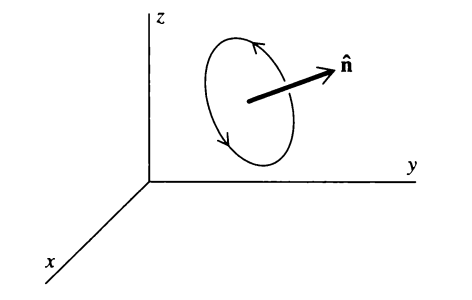
\includegraphics[width=20em]{calc_multi_70_div_curl_lap_06.png}

Çizgi entegrali yardıma yetişiyor. Üç tane eksen üzerinden, o eksenler etrafında
ufak bir dönme yolunun yaptığı işi ayrı ayrı hesaplayabiliriz, ve sonucu aynı
boyutta bir vektörün boyutları olarak kabul edebiliriz, ve vektörün gösterdiği
yön etrafında sağ el kuralı dönüşün nasıl olduğunu tarif eder, vektörün
büyüklüğü ise dönüşün hızını. 

Hatırlarsak yapılan iş $W = \int_{t=a}^{t=b} F \cdot T \ud s$ ile hesaplanır,
$T$ ile $F$'nin üzerinde gidilen eğrinin yansımasına bakıyoruz, $\ud s$ bu
eğrinin ufak bir parçası [9, sf. 1153]. Aynı işlem $F \ud \vec{r}$ ile de
gösterilebilir.

Devam edersek, şimdi diyelim ki $F$'nin ufak bir dikdörtgen etrafında yaptığı
dönüşsel işi, dolaşımını (circulation) hesaplayacağız. Sonra dikdörtgeni limite
götürüp sonsuz küçültünce bir analitik sonuca erişmiş olacağız.

Bu hesabı her eksen için yapmak istiyoruz, önce $z$'den başlayalım, dolaşım $xy$
düzleminde olacak [8, sf. 77].

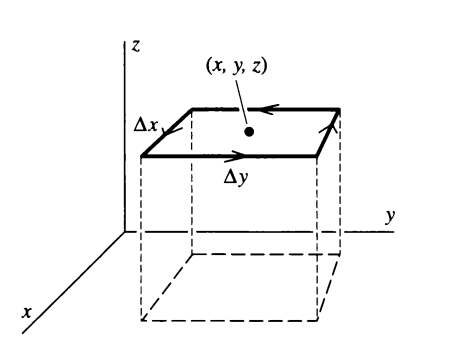
\includegraphics[width=20em]{calc_multi_70_div_curl_lap_07.png}
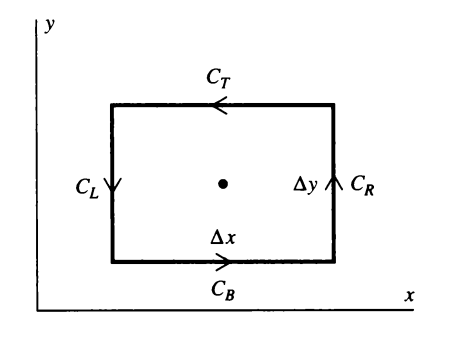
\includegraphics[width=20em]{calc_multi_70_div_curl_lap_08.png}

Önce $C_B$ parçasını hesaplayalım. Üst sağdaki resimde görülüyor, ortaki
noktanın kordinat değeri $x,y,z$, $C_B$ üzerinde $F$'nin bileşeni $F_x$, oradaki
$F_x$ değeri $F_x(x,y-\frac{\Delta y}{2}, z)$. Bu kuvveti $C_B$ boyunca
katedilen yol $\Delta x$ ile çarpıyoruz,

$$
\int_{C_B} F \cdot T \ud s =
\int_{C_B} F_x \ud x \approx
F_x \left( x,y-\frac{\Delta y}{2}, z \right) \Delta x
$$

$C_T$ icin

$$
\int_{C_T} F_x \ud x \approx -F_x \left(x,y+\frac{\Delta y}{2}, z \right) \Delta x
$$

Yukarı ve aşağı gidişi hesaplamadık çünkü o yollar $F_x$'e dik, yapılan iş
sıfır. Üstteki sonuçları toplarsak,

$$
\int_{C_T+C_B} F \cdot T \ud s  = - \left[
F_x \left( x,y+\frac{\Delta y}{2},z \right) -
F_x \left( x,y-\frac{\Delta y}{2},z \right)
\right] \Delta x
$$

$$
= - \dfrac{
\left[
  F_x \left( x,y+\dfrac{\Delta y}{2},z \right) -
  F_x \left( x,y-\dfrac{\Delta y}{2},z \right)
\right]  
}{\Delta y}
\Delta x \Delta y
$$

$\Delta x \Delta y$ carpani tabii ki dikdortgenin alani. Onu sol tarafa alirsak,

$$
\frac{1}{\Delta S}\int_{C_T+C_B} F \cdot T \ud s \approx
- \dfrac{
\left[
  F_x \left( x,y+\dfrac{\Delta y}{2},z \right) -
  F_x \left( x,y-\dfrac{\Delta y}{2},z \right)
\right]  
}{\Delta y}
$$

Benzer analizi dikdörtgenin sağ ve sol tarafına, $C_L$ ve $C_R$ için uygularsak,

$$
\frac{1}{\Delta S}\int_{C_L+C_R} F \cdot T \ud s \approx
- \dfrac{
\left[
  F_y \left( x+\dfrac{\Delta x}{2},y,z \right) -
  F_y \left( x-\dfrac{\Delta x}{2},y,z \right)
\right]  
}{\Delta x}
$$

Son iki sonucu toplarız, $\Delta S$'nin limitini alırız, böylece dikdörtgen
$x,y,z$ noktasına sonsuz küçültülmüş olur, ki bu durumda $\Delta x \to 9$ ve
$\Delta y \to 0$, böylece nihai eriştiğimiz sonuç,

$$
\lim_{\Delta \to 0} \frac{1}{\Delta S} \oint F \cdot T \ud s =
\frac{\partial F_y}{\partial x} - \frac{\partial F_x}{\partial y}
$$

Entegralde $\int$ yerine $\oint$ kullandık ki dolaşım hesabı olduğu daha iyi
belli olsun.

Tabii bu tek eksen, $z$ ekseni etrafındaki dolaşım. Aynı işlemi diğer eksenlere
de uygularsak,

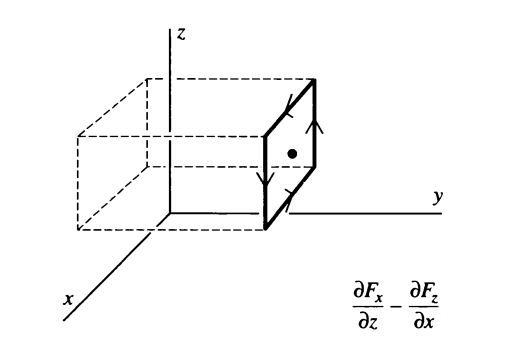
\includegraphics[width=20em]{calc_multi_70_div_curl_lap_09.png}
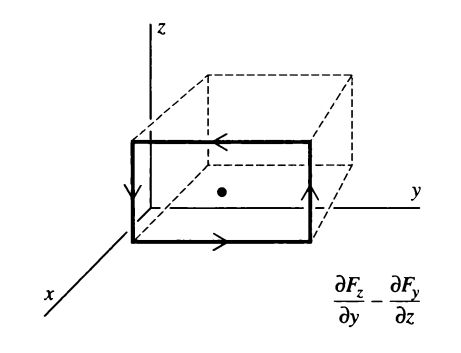
\includegraphics[width=20em]{calc_multi_70_div_curl_lap_10.png}

Tüm bu bileşenleri bir araya koyunca (2)'de gösterilen curl vektörüne ulaşmış
oluyoruz, $z$ ekseni etrafındaki 3. öğe, üstteki soldaki 2. sağdaki 1. öğe,

$$
\curl F = \left[\begin{array}{ccc} 
\dfrac{\partial F_z}{\partial y} - \dfrac{\partial F_y}{\partial z} & 
\dfrac{\partial F_x}{\partial z} - \dfrac{\partial F_z}{\partial x} & 
\dfrac{\partial F_y}{\partial x} - \dfrac{\partial F_x}{\partial y} 
\end{array}\right]
$$

$F_1,F_2,F_3$ yerine $F_x,F_y,F_z$ kullanmış olduk.

Kaynaklar

[1] Strang, {\em Computational Science and Engineering}

\end{document}

